\chapter{Algoritmo genético}

\section{Evolución natural}

La evolución, en relación con la genómica, es el proceso por el cual los organismos vivos cambian con el tiempo a través de cambios en el genoma, esto cambios provocan individuos con rasgos alterados que afectan su supervivencia. Los supervivientes se reproducen y trasmiten estos genes alterados, los cambios que atentan contra la supervivencia de algún individuo, impide la reproducción del mismo \cite{evolucion}.

En la naturaleza, para que exista un proceso evolutivo se deben cumplir las siguientes condiciones:
\begin{itemize}
	\item Una entidad o individuo con la capacidad de reproducción.
	\item Una población de dichos individuos.
	\item Diferencias entre los individuos de la población.
	\item La variedad es un factor que determina el nivel de supervivencia de ese individuo.
\end{itemize}

La evolución afecta los cromosomas, estos son estructuras que transporta la información genómica de una célula a otra, y es mediante la reproducción en donde se combinan los cromosomas de los padres para formar nuevas estructuras \cite{evolucion_2, cromosoma}.

\section{Evolución artificial}

Los algoritmos genéticos simulan el comportamiento evolutivo de una población en donde los mas aptos heredan sus genes a las nuevas generaciones para obtener nuevos resultados.  Este proceso tiene los siguientes pasos:
\begin{itemize}
	\item \textbf{Selección}: Se seleccionan las parejas (o grupos) de individuos de la población con las mejores aptitudes. Este conjunto serán los padres de la nueva generación.
	
	\item \textbf{Cruza}: Se realiza una combinación entre los genomas de las parejas seleccionadas para producir un numero de hijos con códigos genéticos diferentes.
	
	\item \textbf{Mutación}: Sea realiza algún cambio aleatorio en el genoma de cualquier elemento de la nueva población.
	
	\item \textbf{Reemplazo}: Criterio que define que elementos de la nueva generación reemplazaran a la generación anterior.
\end{itemize}

\subsection{Ventajas}

\begin{itemize}
	\item Puede explorar el espacio de soluciones en múltiples direcciones al mismo tiempo.
	\item Realizan una amplia exploración, permitiendo escapar de óptimos locales para conseguir óptimos globales.
	\item Trabajan bien en problemas complejos y cambiantes, así como aquéllos en los que la función objetivo es discontinua, ruidosa, o que tiene muchos óptimos locales, ademas de poder soportar las optimizaciones multi-objetivo.
	\item Cada parte del proceso puede ser implementada por diferentes funciones para mejorar el rendimiento del algoritmo, por ejemplo, existen funciones enfocadas unicamente en la exploración.
	
\end{itemize}

\subsection{Desventajas}

\begin{itemize}
	\item La función objetvo es muy sensible para los algotimos GA, ya que si se elige mal o se define incorrectamente, puede que sea incapaz de encontrar una solución al problema.
	\item La elección de los parámentros (tamaño de la población, cruzamiento, selección de padres, mutación, entre otras más) de los algoritmos GA puede llegar a ser muy complejo. Una mala elección en los parámetros puede provocar un mal desempeño.
	\item Consumen mucho tiempo de ejecución y potencia de cómputo.
	\item Existe el riesgo de encontrarse con una convergencia prematura; es decir, se puede reproducir abundantemente un individuo haciendo que merme la diversidad de la población demasiado pronto, provocando que converja hacia un óptimo local, el cual representa a ese individuo.
\end{itemize}

\subsection{Fenotipo y genotipo}

El \textbf{fenotipo} es la forma que toma la posible solución del problema, como números, cadenas, grafos, tablas, imágenes, etc. El \textbf{genotipo} (también llamado cromosoma) esta construido a partir del fenotipo y representa la codificación de sus características, generalmente como un vector.

\begin{figure}[H]
	\centering
	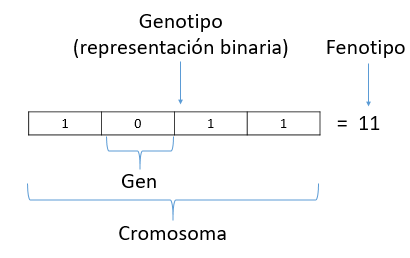
\includegraphics[width=0.75\linewidth]{img/fen_gen.png}
	\caption{Descripción grafica de genotipo, fenotipo, cromosoma y gen del numero ``11''}
	\label{fig:fen_gen}
\end{figure}

\subsection{Modelos generacionales y estacionarios}

En cada paso evolutivo, la cantidad de la población seleccionada y la forma de como se reintegran los nuevos individuos afectan el comportamiento general de la población, la velocidad en como evoluciona y el espacio de exploración para la búsqueda de óptimos globales.

Los \textbf{Modelos generacionales} actualizan la mayor parte de la población, se busca tener evoluciones rápida y una amplia exploración. Para ello se selecciona un pequeño conjunto de individuos y se les aplica los algoritmos de selección, cruza y mutación. Finalmente, mediante el algoritmo de reemplazo se reintegran en la población mediante una función.	

Por otro lado, los \textbf{modelos estacionarios} buscan mantener el equilibrio en la mayor parte de la población experimentando y mezclando un pequeño conjunto.  El cambio es mas lento pero mas estable.